\documentclass{article}
\usepackage{tikz}
\usetikzlibrary{calendar}
\usepackage[utf8]{inputenc}

\title{Rapport intermediaire pour Projet Long}
\author{Nicolas Peneloux, Ymri Scheiner}
\date{15 Mars 2024}

\begin{document}

\maketitle

\section{Introduction}

Notre projet consiste à réaliser un auto tuner, c'est à dire un programme qui recoit en entrée un fichier audio d'une voix, et ressort en sortie une version de cette audio dont les notes sont modifié selon les désirs de l'utilisateur, sans modifier le reste de l'audio. Grossièrement, nous pouvons diviser cela en 2 : 
\begin{itemize}
  \item Pitch Tracking : récupérer les différentes notes de l'audio
  \item Pitch Correction : changer les notes vers les hauteurs souhaitées
\end{itemize}
\par 

\subsection*{Métriques}
Pour mesurer le succès de notre projet, nous utiliserons les métriques suivantes :




\section{Implémentation}

Nous réalisons ce projets en \textbf{Rust}, en nous appuyant sur \textbf{l'algorithme FFT (Fast Fourier transform)} pour représenter l'audio sous une forme de données pragmatiques pour notre projet, une méthode très courante pour le traitement de signal. 
Nous utilisons également d'autres algorithmes basés sur cette technologie tel que l'algorithme PIN pour la section pitch correction.
\par
En terme de modules ou packages, la strudcture interne du projet est très simple avec un fichier par tâche, a utiliser dans un main.
Nous utilisons quelques packages de Rust pour certaines tâches auxiliaires au projet tel que la création de l'interface graphique, ou la manipulation/création de fichier midi.


\section{Jalons}

\subsection{Tâches à Réaliser}

Nous avons divisé le projet dans sa globalité en 3 grosse tâches, à savoir 
\begin{itemize}
  \item l'implémentation de l'algorithme FFT pour permettre de transformer des fichiers audio en données utilisables
  \item l'implémentation du pitch tracking
  \item l'implémentation de la pitch correction
\end{itemize}

Viennent ensuite s'ajouter des tâches auxiliaires telles que la mise en place de tests, la création de l'interface graphique etc...

\subsection{Tâches Terminées}

Les deux première tâches parmi celles énumérées au dessus ont été réalisés, ainsi que quelques tâches auxiliaires. Des tests ont été mit en place pour la partie FFT, et l'interface utilisateur a déjà été conçue.

\subsection{Organisation Temporelle}

Il manque ainsi la partie pitch correction et l'implémentation de tests pour la partie pitch tracking. 
\par
Idéalement, nous pouvons consacrer 2 semaines sur l'implémentations des tests et les semaines restantes pour coder la partie pitch correction.


\subsection*{Calendrier Visuel}

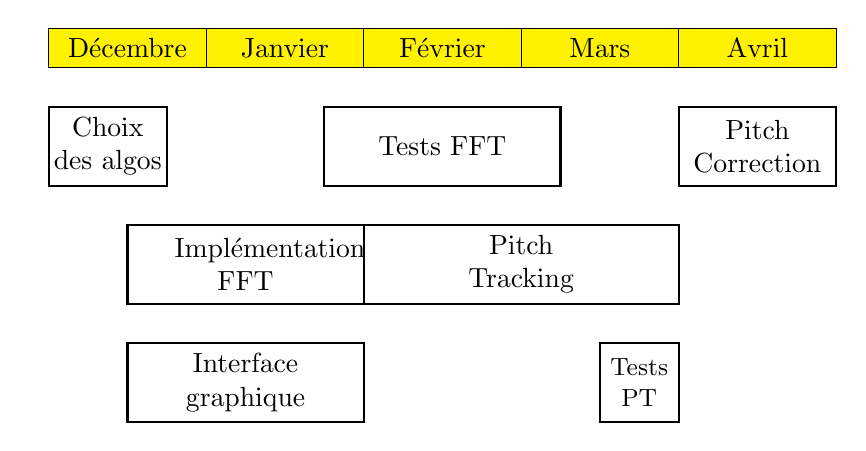
\begin{tikzpicture}
%Mois
\draw[fill=yellow] (0,0) rectangle (2,0.5) node[pos=.5] {Décembre};
\draw[fill=yellow] (2,0) rectangle (4,0.5) node[pos=.5] {Janvier};
\draw[fill=yellow] (4,0) rectangle (6,0.5) node[pos=.5] {Février};
\draw[fill=yellow] (6,0) rectangle (8,0.5) node[pos=.5] {Mars};
\draw[fill=yellow] (8,0) rectangle (10,0.5) node[pos=.5] {Avril};

%Tâches
\draw[thick] (0,-0.5) rectangle (1.5, -1.5) node[pos=.5, text width=1.8cm, align=center] {Choix des algos};
\draw[thick] (1,-2) rectangle (4, -3) node[pos=.5, text width=1.8cm, align=center] {Implémentation FFT};
\draw[thick] (1,-3.5) rectangle (4, -4.5) node[pos=.5, text width=1.8cm, align=center] {Interface graphique};
\draw[thick] (3.5,-0.5) rectangle (6.5, -1.5) node[pos=.5, text width=1.8cm, align=center] {Tests FFT};
\draw[thick] (4,-2) rectangle (8, -3) node[pos=.5, text width=1.8cm, align=center] {Pitch Tracking};
\draw[thick] (7,-3.5) rectangle (8, -4.5) node[pos=.5, text width=1cm, align=center, font=\small] {Tests PT};
\draw[thick] (8,-0.5) rectangle (10, -1.5) node[pos=.5, text width=1.8cm, align=center] {Pitch Correction};


\end{tikzpicture}

\section*{Problèmes rencontrés}
Nous avons d'abord mit du temps a trouver un sujet accepté, mais aussi après dans la réalisation du projet jusqu'a maintenant. Les difficultés majeures que nous avons rencontrées sont 
\begin{itemize}
   \item l'utilisation de rust que nous avons tout les deux du apprendre sur le tas
  \item la compréhension théorique des algorithmes et technologies que nous utilisons car c'était notre premier projet dans le domaine du traitement audio
  \item le choix des algorithmes a utiliser car en rapport avec le point précédent, les différencens peuvent être nuancées et dure a saisir sans en connaître les tenants et aboutissants
\end{itemize}

\end{document}
